\section{Objectives and handout mapping}

Handout PDF pages 62--64 are covered by Step 1 FF/TT/SS delay and power tests, Q1 mixed-corner ratioed-logic tests, and Q2 reverse-junction leakage comparisons. Eight decks contain 17 executed analyses.

The user-selected CIC 0.18 µm, 1.8 V devices replace the handout example at 0.25 µm and 2.5 V. These results do not reproduce the original numerical table. The handout inverter dimensions Wn/Wp/L = 0.6/1.8/0.25 µm are retained, with nominal supply adapted to 1.8 V. The explicit 1.98 V and 1.62 V conditions implement the teaching ±10\% sweep, not voltage-reliability qualification.

\section{Methods and reproducible data}

HSPICE S-2021.09 completed all analyses without reported warnings, errors, or failed measurements. Input period is 4 ns with 0.2 ns edges and a 10 fF load. Delay uses half-supply crossings on the second transition, with $t_p=(t_{pHL}+t_{pLH})/2$. Power is average supply input power from 4 to 12 ns. Additional FF and SS runs at 1.8 V and 25°C isolate process variation.

Decks 01--03 are transient tests and 04--08 are DC tests. Public decks contain only a \texttt{MODEL\_SETUP\_REQUIRED} comment and corner label. Neither model content nor loading paths are distributed; local setup is required before running. Figures use actual simulation data, with per-case CSV, measurement JSON, and comparison CSV files in \texttt{results/}.

\section{Process, voltage, and temperature results}

\begin{center}\small
\begin{tabular}{lrrrr}
\toprule
Corner & V (V) & T (°C) & $t_p$ (ps) & $P$ (µW) \\
\midrule
TT & 1.8 & 25 & 87.110 & 11.946 \\
FF & 1.98 & 0 & 69.853 & 15.239 \\
SS & 1.62 & 115 & 159.081 & 10.150 \\
FF & 1.8 & 25 & 77.092 & 12.240 \\
SS & 1.8 & 25 & 129.262 & 12.232 \\
\bottomrule
\end{tabular}
\end{center}

\begin{figure}[htbp]\centering
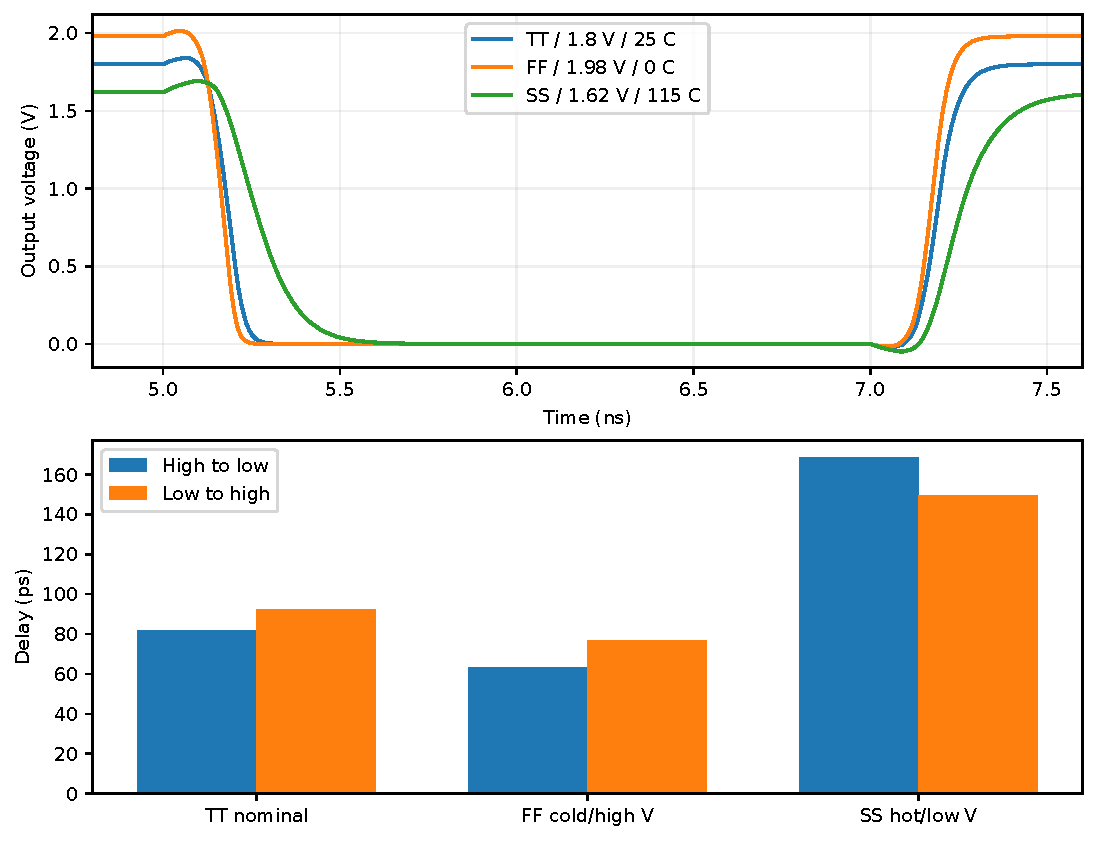
\includegraphics[width=.93\linewidth]{figures/pvt.pdf}
\caption{Outputs and both propagation delays for the three combined PVT cases.}
\end{figure}

Combined-corner mean delays for FF, TT, and SS are 69.853, 87.110, and 159.081 ps, with powers of 15.239, 11.946, and 10.150 µW. The faster combined corner is faster and consumes more power here. At fixed supply and temperature, however, SS power is 12.232 µW, slightly above TT. Power cannot be ranked universally by fast/slow labels; input frequency, load switching, and short-circuit current all matter.

\section{Q1: mixed corners in ratioed logic}

The pseudo-NMOS PMOS is always on with W/L = 0.6/0.5 µm; the NMOS is 0.6/0.25 µm. Its low output is determined by competing pull-up/down currents, so SF and FS must be checked. The table uses 1.8 V, 25°C, and input 1.8 V. Static CMOS low outputs are near zero, while pseudo-NMOS retains a measurable DC voltage and power.

\begin{center}\small
\begin{tabular}{lrr}
\toprule
Corner & $V_{OL}$ (V) & $P_{static}$ (µW) \\
\midrule
TT & 0.063495 & 87.209 \\
FF & 0.061252 & 102.027 \\
SS & 0.100317 & 62.364 \\
SF & 0.172730 & 101.363 \\
FS & 0.077670 & 93.937 \\
\bottomrule
\end{tabular}
\end{center}

\begin{figure}[htbp]\centering
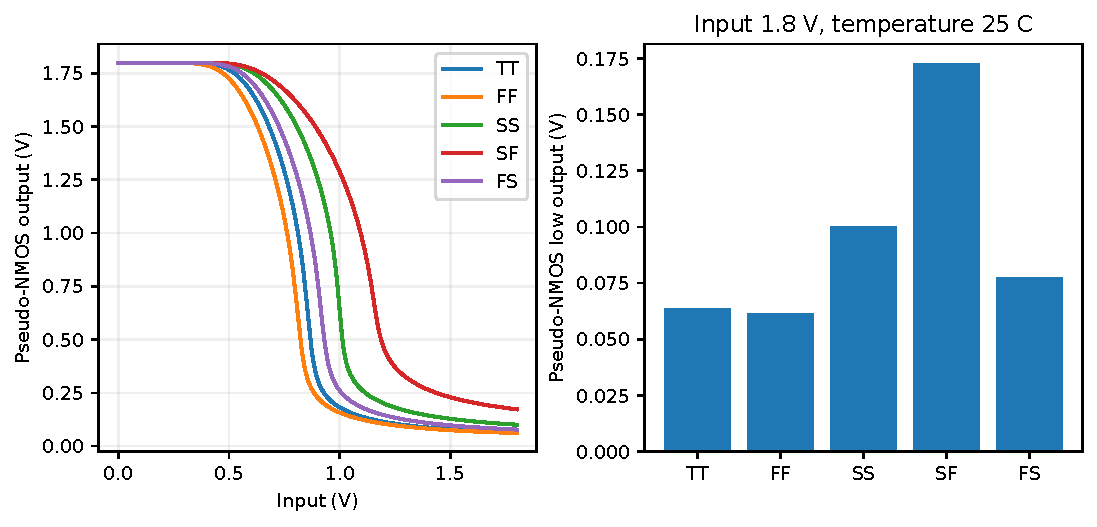
\includegraphics[width=.93\linewidth]{figures/ratioed.pdf}
\caption{Mixed corners change the worst low-output condition for the ratioed circuit.}
\end{figure}

SF gives VOL = 0.172730 V, exceeding FF, TT, and SS, so checking only the three same-direction corners would miss this worst result. Ratio-less static CMOS does not make SF/FS universally irrelevant: switching threshold, duty cycle, noise margins, and other asymmetric requirements may still be limited by mixed corners.

\section{Q2: reverse-junction leakage}

Separate NMOS and PMOS test devices tie D, S, and G together, setting $V_{DS}=V_{GS}=0$ while reverse-biasing both D/B and S/B junctions. Each junction has area 0.15 µm$^2$, perimeter 1.7 µm, and reverse bias 1.8 V. Body current measures the two-junction total. Whole-inverter off-state current is not mislabeled as a single junction current.

GMIN = GMINDC = $10^{-18}$ S contributes $2(1.8)(10^{-18})=3.6\times10^{-18}$ A across the two junctions; this known numerical contribution is explicitly subtracted from raw results. A TT 25°C rerun at $10^{-15}$ S yields matching corrected NMOS/PMOS currents. Raw and corrected values are retained in CSV. At 0°C, the raw values are tiny and the numerical contribution is significant.

\begin{center}\small
\begin{tabular}{lrr}
\toprule
T (°C) & N (A) & P (A) \\
\midrule
0 & 4.7115e-18 & 2.8546e-18 \\
25 & 4.2894e-16 & 2.5988e-16 \\
115 & 4.9026e-11 & 2.9704e-11 \\
\bottomrule
\end{tabular}
\end{center}

\begin{figure}[htbp]\centering
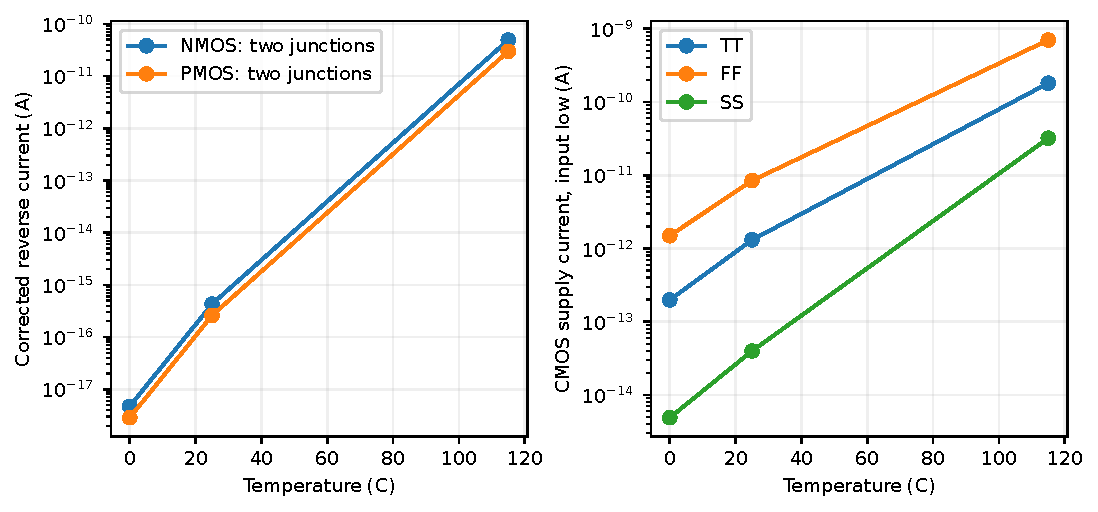
\includegraphics[width=.93\linewidth]{figures/leakage.pdf}
\caption{Left: corrected junction leakage. Right: inverter supply leakage; these are different quantities.}
\end{figure}

For this model and identical temperature/junction geometry, isolated junction currents are identical across TT/FF/SS, while temperature has a very large effect. Inverter supply leakage does vary with corner: at 25°C with low input, FF/TT/SS are 8.429/1.308/0.03975 pA. Different leakage mechanisms therefore cannot be assumed to share the same FF > TT > SS ranking.

\section{Conclusions and limits}

The corner delay/power experiment and both questions are completed. Results apply to the selected model, geometry, load, and stated stimulus. They do not establish reproduction of the original 0.25 µm values, complete PVT signoff, statistical yield, or post-layout behavior. Other labs retain their original model.
